\documentclass{CInf_practice}

\sheet{12}{Stoppuhr auf dem ATmega16}

\lstset{language={[avr8avra]Assembler},
        morecomment=[n]{/*}{*/},
        morecomment=[l]{//},
     }
\usepackage{marvosym}

\begin{document}
\cinftitle

Das gesamte Programm befindet sich am Ende der Abgabe.
Für die einzelnen Teilaufgaben ist jeweils der wichtigste Codeabschnitt
direkt erwähnt. Dabei sind aber ggf. Sprungadressen, Compilerdirektiven u.ä.
nicht direkt aufgeführt, wenn sie an anderer Stelle im Code stehen. Der gesamte
Code am Ende hält diese Befehle dann bereit.

Die Header-Datei des letzten Aufgabenblatts wurde hier (korrigiert) wieder 
verwendet, sie befindet sich noch nach dem Programmcode ganz am Ende.

\ex{Systemstruktur}{6 + 4}


\subex{Modulbild}
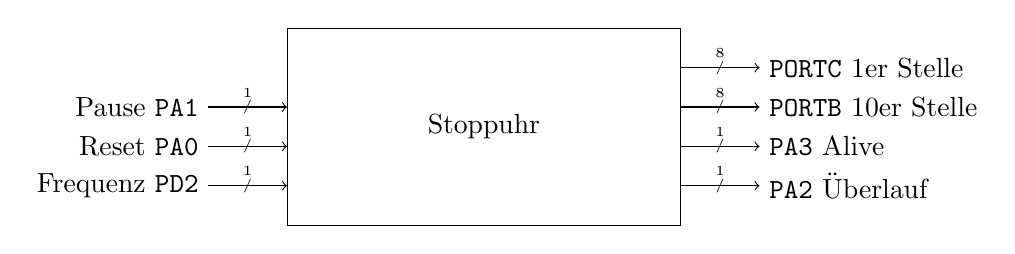
\begin{tikzpicture}
  \def\instart{2}
  \def\outstart{8}
  \newcounter{inbus}
  \newcounter{outbus}
  \def\bus#1#2#3#4#5{
    \def\xval{\ifnum#1=0{\instart}\else{\outstart}\fi}
    \draw[->] (\xval, #2) node[left] {\ifnum#1=0{#5 {\tt #4}}\fi} 
          -- node{\tiny /} node[above]{\tiny #3} 
          ++(1,0) node[right] {\ifnum#1=1{{\tt #4} #5}\fi};
  }
  \def\inbus#1#2#3{
    \stepcounter{inbus}
    \bus{0}{.5*\value{inbus}}{#2}{#1}{#3}
  }
  \def\outbus#1#2#3{
    \stepcounter{outbus}
    \bus{1}{.5*\value{outbus}}{#2}{#1}{#3}
  }
  \def\baseheight{\ifnum\value{inbus}>\value{outbus} \value{inbus}\else\value{outbus}\fi}
	
  \inbus{PD2}{1}{Frequenz}
  \inbus{PA0}{1}{Reset}
  \inbus{PA1}{1}{Pause}
  \outbus{PA2}{1}{Überlauf}
  \outbus{PA3}{1}{Alive}
  \outbus{PORTB}{8}{10er Stelle}
  \outbus{PORTC}{8}{1er Stelle}
  
  \draw (\instart+1, 0) rectangle node{Stoppuhr} (\outstart,.5*\baseheight+.5);
\end{tikzpicture}

\subex{Registerbelegungsplan}
\begin{tabular}{l|l|l}
\bf Register & \bf Name & \bf Funktion \\\hline
R16 & tmp & Temporäres Register, universell eingesetzt \\
R17 & time & aktuelle Zeit der Stoppuhr, hält kompakten BCD-Wert \\
X & X & Adressregister, für Table-Initialisierung und Lookups
\end{tabular}

\ex{Konfiguration der I/O-Ports}{10}
\lstinputlisting[linerange={58-81}]{stopwatch.asm}


\ex{Ausgabe der 7-Segment-Codes}{10}
\lstinputlisting[linerange={119-145}]{stopwatch.asm}
\lstinputlisting[linerange={173-195}]{stopwatch.asm}


\ex{Hauptprogramm}{10}
\lstinputlisting[linerange={348-351,356-365,374-375}]{stopwatch.asm}


\ex{Polling vs. Interrupt}{4 + 10 + 4 + 6 + 4}

\subex{Polling}
Achtung, das Polling ist bereits auskommentiert, um den Änderungen aus 
Teilaufgabe d) gerecht zu werden.

\lstinputlisting[linerange={359-374}]{stopwatch.asm}

\subex{\texttt{COUNT\_UP}}
\lstinputlisting[linerange={212-231}]{stopwatch.asm}

\subex{\texttt{ISR\_CLOCK}}
\lstinputlisting[linerange={242-253}]{stopwatch.asm}

\subex{\texttt{INIT\_EXT\_INTERRUPT}}
Die Änderungen im Hauptprogramm sind das Auskommentieren des Pollings sowie
der Aufruf der \texttt{INIT\_EXT\_INTERRUPT}-Routine, wie im Code am Ende der 
Abgabe zu sehen ist.

Der Aufruf von \texttt{INIT\_EXT\_INTERRUPT} im Hauptprogramm ist ebenfalls 
auskommentiert, um Aufgabe 6b) gerecht zu werden.

\lstinputlisting[linerange={266-282}]{stopwatch.asm}

\subex{Vorteile Interrupts}
Die Stopp-Uhr ist genauer, da sie (mehr oder weniger) unabhängig vom 
restlichen Programm korrekt erhöht wird, und nicht nur dann, wenn gerade ein 
Polling ansteht. Außerdem kann so ggf. komplett anderer Code ausgeführt werden,
und trotzdem \emph{im Hintergrund}, also nebenläufig, die Stoppuhr laufen.

\ex{T/C0-Interrupt}{6 + 14}
\subex{Prescale-Faktor}
Der Zusammenhang zwischen Prescale-Faktor $P$, Frequenz $F$ und Anzahl Bits 
des Zählregisters $B$ lässt sich wie folgt veranschaulichen:
\begin{align*}
\frac{F}{P} = 2^B Hz\\
\end{align*}
Daraus ergibt sich für $F = 2^{15} Hz$ und $B = 8$:
\begin{align*}
\frac{2^{15} Hz}{P} = 2^8 Hz \equiv P = \frac{2^{15} Hz}{2^8 Hz} = 2^7 = 128
\end{align*}
Die resultierende Auflösung ist dann $\frac{1 s}{2^7} = 0.0078125 s = 7.8125 ms$.

Der ATmega16 unterstützt die Prescale-Faktoren $8, 64, 256$ und $1024$. Wir 
müssen einen wählen, der größer ist als $128$, damit unser Zähler nicht 
ungewollt überläuft. $256$ bietet sich deshalb an. Der resultierende 
Vergleichswert ist $\frac{2^{15} Hz}{256 Hz} = 2^7 = 128$.

\subex{\texttt{INIT\_TCO\_INTERRUPT}}
Abgesehen von der Konfiguration an den korrekten Stellen (u.a. Interrupt-
Vector-Table und Mainprogram) müssen keine Änderungen vorgenommen werden.

\lstinputlisting[linerange={301-323}]{stopwatch.asm}

\newpage
\ex{Nebenläufigkeiten}{4 + 4 + 4}
In allen drei Fällen steht zu Beginn die Initialisierungsphase. Anschließend
verläuft im Polling-Fall das Programm vollständig sequentiell, mit einer 
Erhöhung des Counters bei einem positiven Polling Ergebnis. Im Fall des 
externen Interrupts wird nach der Initialisierungsphase immer dann {\tt COUNT\_UP}
nebenläufig ausgeführt, wenn ein Interrupt von außen vorliegt. Im letzten Fall
zählt im Hintergrund nebenläufig der T/C0-Zähler mit und bei erreichtem Compare-Value
wird nebenläufig {\tt COUNT\_UP} ausgeführt.

\begin{ctabular}{c|c|c}
\subex{Polling}&
\subex{Externer INT0 Interrupt}&
\subex{Interner T/C0-Interrupt}\\
sequentiell & bei Interrupt nebenläufig & Zähler \& Interrupt nebenläufig \\
\tikz{
  \draw[->] (1.25,5.5) -- ++(0,-.5);
  \foreach \y/\val in {5/INIT,4.5/Loop:,4/\ (RESET),3.5/\ SSEG\_OUT,3/\ POLL,2.5/\ (COUNT\_UP),2/\ JMP Loop}{
    \draw[thin] (0,\y) rectangle node[text width=2cm] {\small\tt \val} ++(2.5,-.5);
  }
  \draw[opacity=0] (0,0) -- (0,-.5); % dummy to move this graph up
} & 
\tikz{
  \draw[->] (1.25,5.5) -- ++(0,-.5);
  \foreach \y/\val in {5/INIT,4.5/Loop:,4/\ (RESET),3.5/\ SSEG\_OUT,3/\ JMP Loop}{
    \draw[thin] (0,\y) rectangle node[text width=2cm] {\small\tt \val} ++(2.5,-.5);
  }
  \draw[->] (2.5,4.75) -| (1+2.7,4.5-.5);
  \foreach \y in {3.5,2,1,.5} {
    \draw[<-] (4.7,\y-.25) -- ++(.4,0);
  }
  \foreach \y/\val in {4/,3.5/COUNT\_UP,3/,2.5/,2/COUNT\_UP,1.5/,1/COUNT\_UP,.5/COUNT\_UP,0/}{
    \draw[thin] (2.7,\y) rectangle node[text width=1.7cm] {\small\tt \val} ++(2,-.5);
  }
} & 
\tikz{
  \draw[->] (1.25,5.5) -- ++(0,-.5);
  \foreach \y/\val in {5/INIT,4.5/Loop:,4/\ (RESET),3.5/\ SSEG\_OUT,3/\ JMP Loop}{
    \draw[thin] (0,\y) rectangle node[text width=2cm] {\small\tt \val} ++(2.5,-.5);
  }
  \draw[->] (2.5,4.75) -| (.75+2.7,4);
  \foreach \y in {4,3.5,3,2.5,2,1.5,1,.5,0}{
    \draw[thin] (2.7,\y) rectangle node[text width=1.4cm] {\small\tt TCNT+1} ++(1.5,-.5);
  }
  \foreach \y in {3.5,2.5,1.5,.5} {
    \draw[->] (2.7+1.5,\y-.25) -- ++(.4,0);
  }
  \foreach \y/\val in {4/,3.5/COUNT\_UP,3/,2.5/COUNT\_UP,2/,1.5/COUNT\_UP,1/,.5/COUNT\_UP,0/}{
    \draw[thin] (2.7+1.5+.4,\y) rectangle node[text width=1.7cm] {\small\tt \val} ++(2,-.5);
  }
} \\
\end{ctabular}

\newpage
{\large\textbf{Vollständiger Programmcode}}
\lstinputlisting{stopwatch.asm}

\newpage
{\large\textbf{\texttt{init\_header.inc}}}
\lstinputlisting{init_header.inc}

\end{document}
